\chapter{Accelerated MPI Collective Using Software-Defined Networking}\label{sec:iii}

\section{Introduction}\label{sec:iii-introduction}

As described in Section~\ref{sec:i-mpi}, communication primitives defined in
MPI can be roughly categorized into point-to-point communication, collective
communication and one-sided communication. Out of these three categories, this
dissertation particularly focus on accelerating collective communication
because of its significant impact to the application performance. In fact, a
recent analysis of MPI usage on a production HPC system has revealed that
approximately 34\% of the total core-hours of the system are expended in MPI
communication and 66\% of the total MPI communication time is spent in
collective communication~\autocite{Chunduri2018}. This fact clearly indicates
that reducing the time of collective communication is of great importance.

MPI collectives require intensive communication among multiple compute node
pairs. However, some compute node pairs communicate less, whereas other pairs
have to communicate much more. Because of this imbalance, even in the case
where the interconnect of a cluster system has multiple redundant routes
between compute nodes, the packet flow generated from MPI collectives could
collide on a single link of the interconnect without any control of packet
flow.

This chapter aims at accelerating MPI collectives by dynamically controlling
the packet flow in the interconnect. In particular, a cluster system deployed
with an interconnect that contains multiple redundant routes is targeted. This
is because the majority of interconnects today are provisioned with redundant
routes to improve the bisection bandwidth and fault tolerance. Specifically,
this research specifically focuses on fat-tree. This research designs and
implements a framework that effectively makes use of redundant routes by
dynamically controlling the packet flow in the interconnect using SDN
described in Section~\ref{sec:i-sdn}.

The rest of this chapter is organized as follows.
Section~\ref{sec:iii-background} reviews conventional traffic balancing
methods and analyzes their problems. Subsequently, the goal of this chapter is
clarified. In Section~\ref{sec:iii-proposal}, the design and implementation of
the proposed architecture of SDN-enhanced MPI\_Allreduce is presented. In
Section~\ref{sec:iii-evaluation}, an evaluation on a cluster system is
conducted to verify the feasibility of the proposed framework.
Section~\ref{sec:iii-related-work} discusses related works.
Section~\ref{sec:iii-conclusion} concludes this chapter and discusses
challenges for further improving the practicality of our proposed framework.

\section{Research Objective}\label{sec:iii-background}

MPI collective operations require a large number of simultaneous communication
among multiple process pairs. However, some compute node pairs communicate
less, whereas other pairs have to communicate much more. When the underlying
network of the cluster system that interconnects with the compute nodes has a
full-bisection bandwidth, the imbalance of source and destination in
communication would not be a problem although structuring this type of a
network is hard to scale out due to economic and physical
restrictions~\autocite{Al-Fares2008}. Under the assumption that the network is
oversubscribed, the shortage of available bandwidth could give rise to a
serious problem.

Suppose a cluster system of four compute nodes interconnected with a
two-tier fat-tree topology as illustrated in Fig.~\ref{fig:problem-routing1}.
Fat-tree is a network topology that has multiple redundant routes between the
upper layer switches and lower layer switches. By distributing traffic among
these redundant routes, it is possible to gain higher bisection bandwidth
compared to a simple tree topology.

The traffic load balancing algorithm deployed on the interconnect becomes
important on such an interconnect. For example, suppose compute node 1 is
sending data to node 3, and node 2 is sending different data to node 4 at the
same moment in Fig.~\ref{fig:problem-routing1}. If those two communications
are routed within the exact same route, link contention could happen. When
these two communications are routed so that they make use of the redundant
routes as depicted in Fig.~\ref{fig:problem-routing2}, link contention can be
avoided.

\begin{figure}
    \centering
    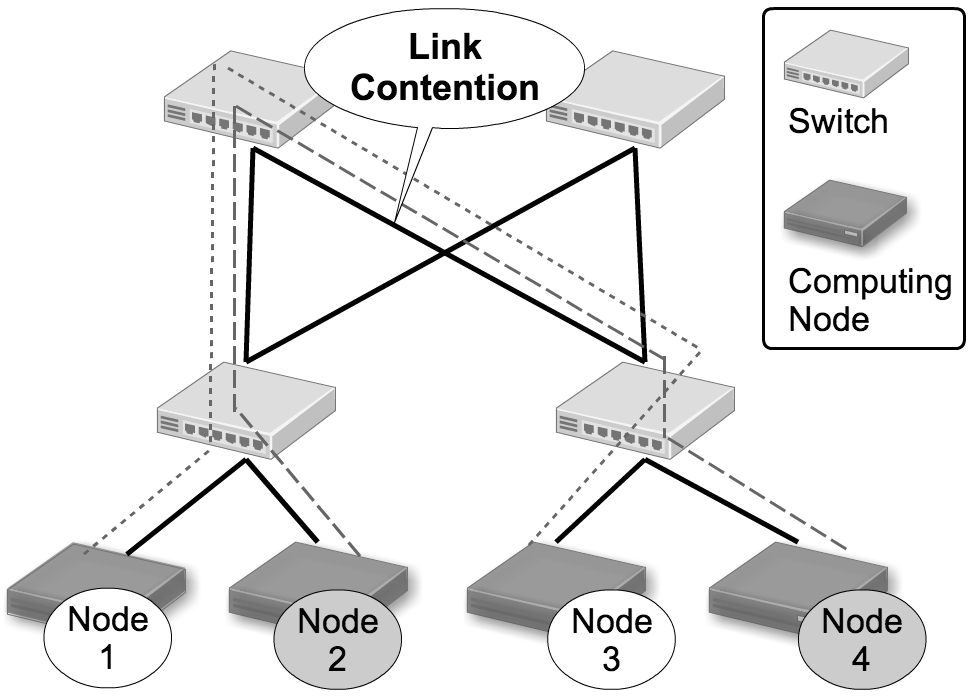
\includegraphics[width=.6\linewidth]{problem-routing2.png}
    \caption{Link Contention on Fat-tree}%
    \label{fig:problem-routing1}
\end{figure}

\begin{figure}
    \centering
    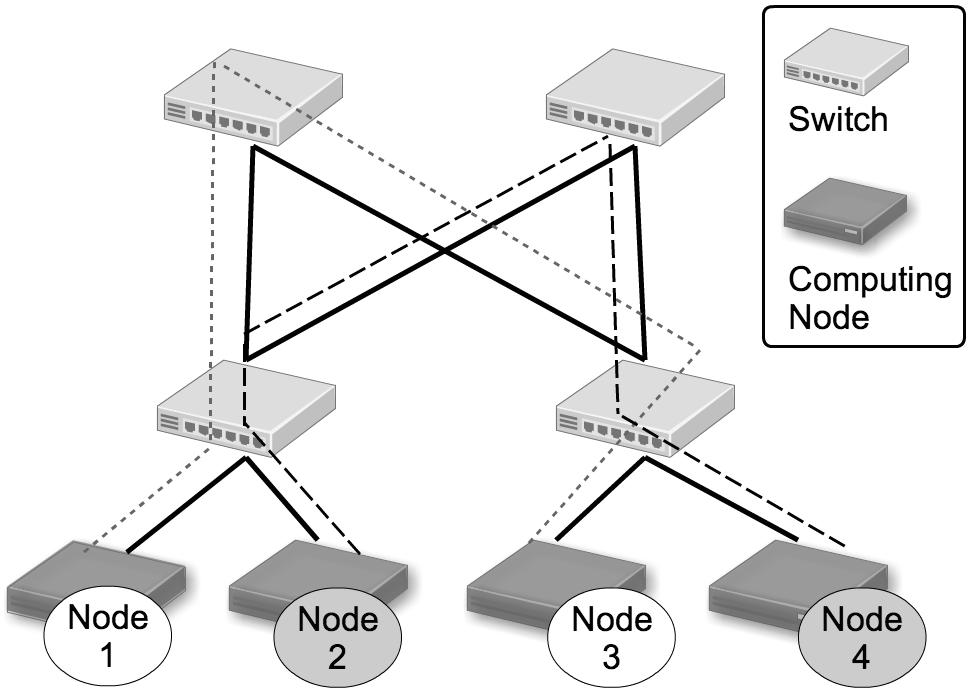
\includegraphics[width=.6\linewidth]{problem-routing1.png}
    \caption{Load Balancing Routes on Fat-tree}%
    \label{fig:problem-routing2}
\end{figure}

Various algorithms for balancing traffic in a network with redundant routes
have been proposed. Equal-Cost Multi-Path routing (ECMP)~\autocite{ecmp} is a
standardized load balancing strategy mainly used in L3 switches. For each
communication between two compute nodes, if multiple equal cost routes are
available, ECMP selects one route from among them. The decision on which route
to use is based on the header fields (\emph{e.g.} source and destination
addresses) of each packet. A hash function is applied to the header fields to
generate the corresponding hash value for the header fields, where every value
in the hash value space are evenly assigned to one of the equal cost routes.

InfiniBand~\autocite{Buyya2009} is a computer network communication link
commonly used in the area of HPC and a data center. InfiniBand supports
multiple routing methods. One of those methods is a min-hop routing
algorithm, which calculates the minimum hop route between every
compute node pair. If multiple minimum hop routes for a single
compute node pair are available, the algorithm assigns a route so that
usage among links is equalized.

The problem of these existing conventional load balancing mechanisms is
that they never consider the communication pattern of MPI applications. In
general, MPI applications cannot retrieve the usage information of the
underlying network nor control it. Meanwhile, MPI communication in an MPI
application usually shows a strong locality where each process communicates
with a limited number of processes. This non-uniform communication pattern may
cause an inequality of link usage that decreases available bandwidth between
compute nodes. Ultimately, this decrease of available bandwidth can lead to
the performance degradation of MPI applications.

From the observations above, an application-aware network control mechanism
which recognizes the communication pattern needed by MPI collectives is
essential. Also, the mechanism must effectively utilize the bandwidth of each
link by distributing the traffic among redundant routes. Therefore, this
research leverage Software-Defined Networking (SDN) to enable such dynamic
control of packet flow depending on the communication patterns of MPI
applications.

In particular, this research focuses on accelerating MPI\_Allreduce.
MPI\_Allreduce is one of the most frequently used and time-consuming
collective communication functions of MPI\@~\cite{Chunduri2018}.
This collective communication reduces values from all
processes with an operator and broadcasts the result of the reduction to every
process. More specifically, suppose there are $n$ processes in a communicator
and each process with rank $i$ ($0 \leq i < n$) has $l$ values $x_i^0, x_i^1,
\dots, x_i^l$. After MPI\_Allreduce is completed, all processes have values
$y^0, y^1, \dots, y^l$ where $y^j = x_0^j \oplus x_1^j \oplus \dots \oplus
x_{n-1}^j$ and $\oplus$ is the operator used for reduction. The operator can
be any user-defined associative operator or one of the pre-defined operators
such as sum, product, or maximum. Figure~\ref{fig:mpi-allreduce} shows an
example where four processes each having five values call MPI\_Allreduce with
the sum operator.

\begin{figure}
    \centering
    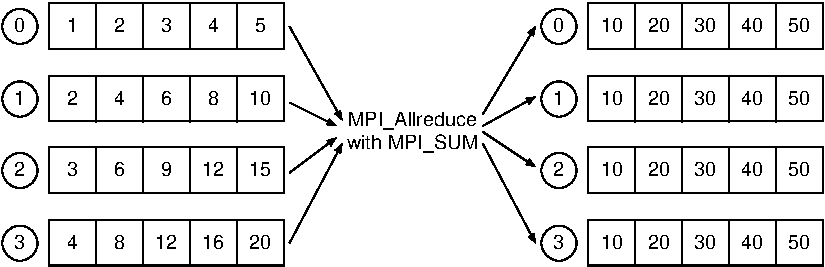
\includegraphics{mpi-allreduce}
    \caption{Effect of MPI\_Allreduce}%
    \label{fig:mpi-allreduce}
\end{figure}

One of the use cases of MPI\_Allreduce is parallel Conjugate Gradient~(CG)
method. CG method is an iterative algorithm to solve a system of linear
equations $Ax = b$ whose coefficient matrix $A$ is positive-definite and
symmetric. In the parallel CG method, a significant amount of time is spent in
MPI\_Allreduce to compute the inner product of
vectors~\autocite{Kandalla2012}. Another use case is parallel Stochastic
Gradient Descent~(SGD). SGD is a continuous optimization algorithm that
minimizes an objective function $f$ parameterized by $w$ for a given set of
input $S$. SGD incrementally updates $w$ in the following way: $w^{t+1}=w^t-
\eta \nabla f(w^t; z^t)$ where $w^t$ is the parameter for the $t$-th
iteration, $z^t$ is an input data randomly sampled from $S$, and $\eta$ is a
small constant. In parallel SGD, the gradient $\nabla f(w^t; z^t)$ is computed
in parallel by each process using different samples. Subsequently,
MPI\_Allreduce is used to compute the average of the individual gradients
computed by all processes.

This research attempts to accelerate MPI\_Allreduce on a cluster system with a
fat-tree interconnect. The dynamic network controllability of SDN is
integrated with MPI in order to mitigate link contention. The speedup of
MPI\_Allreduce based on the proposed framework is evaluated.

\section{Proposal}\label{sec:iii-proposal}

This section presents the proposed framework for accelerating MPI collectives.
First, the basic idea behind the proposed framework is outlined. After that,
the design and implementation of the framework is described in detail.

\subsection{Basic Idea}

The motivation behind the proposed framework is to improve the inefficient communication
in MPI in order to enhance the performance of MPI applications. The fact that
MPI applications are unable to retrieve the usage of the underlying network
results in a potential inefficiency in terms of communication. One of such
inefficiencies is the inequality of link usage among links. Since the
bandwidth of a link is limited, an inequality of link usage can cause
congestion in heavy-loaded links. Therefore, this research focuses on the
inequality of the link usage among the interconnect of a cluster system.

In this chapter, redundant routes in the interconnect are used to mitigate the
inequality of link usage, based on an assumption that the cluster system has a
fat-tree interconnect. Through this traffic distribution, contention in the
links is expected to be alleviated, which as a result speeds up communication.

\subsection{Design of Collective Acceleration Framework Using SDN}%
\label{sec:iii-design}

The proposed framework is composed of three modules. These three modules are
SDN controller, LLDP~(Link Layer Discovery Protocol)~\autocite{lldp} daemon
and SDN MPI library. They are deployed onto a cluster system as illustrated in
Fig.~\ref{fig:proposal-placement}. The SDN controller is designed to be
deployed onto the management node of a cluster system. The management node is
used for controlling the whole cluster system such as deploying jobs to the
system. The LLDP daemon is designed to run in the background on all compute
nodes. The SDN MPI library is a library that needs be statically linked to MPI
applications at compile time.

Although each compute node can run one or more MPI processes, in this chapter,
it is assumed that each compute node runs only a single MPI process. This is a
reasonable assumption since many applications nowadays leverage \emph{hybrid
parallelism}, which combines distributed memory programming and shared memory
programming. Under the hybrid parallelism model, the application starts a
single MPI process per node and then spawns a thread for each socket or core
on the node. After that, the application uses MPI for intra-node communication
and threading frameworks such as OpenMP for intra-node communication.

\begin{figure}
    \centering
    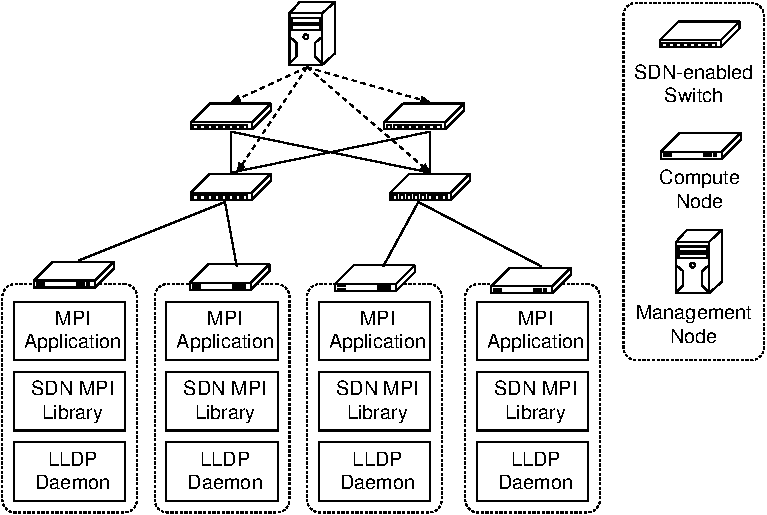
\includegraphics{sdn-mpi-arch}
    \caption{Placement of the Modules Composing SDN-enhanced MPI\_Allreduce}%
    \label{fig:proposal-placement}
\end{figure}

The interaction among these modules is roughly divided into two phases: the
initialization phase at the MPI application startup and the main phase at each
MPI collective call. Figure~\ref{fig:proposal-sequence} is a UML sequence
diagram that illustrates how these modules cooperate with each other.
MPI\_Init is the MPI function that initializes the MPI execution environment,
which must be called on the application startup. After MPI\_Init finishes, all
MPI processes notify their own IP address and MPI rank number to the SDN
controller. This information obtained from MPI processes is held by the
controller until the execution of the MPI application finishes.

\begin{figure}
    \centering
    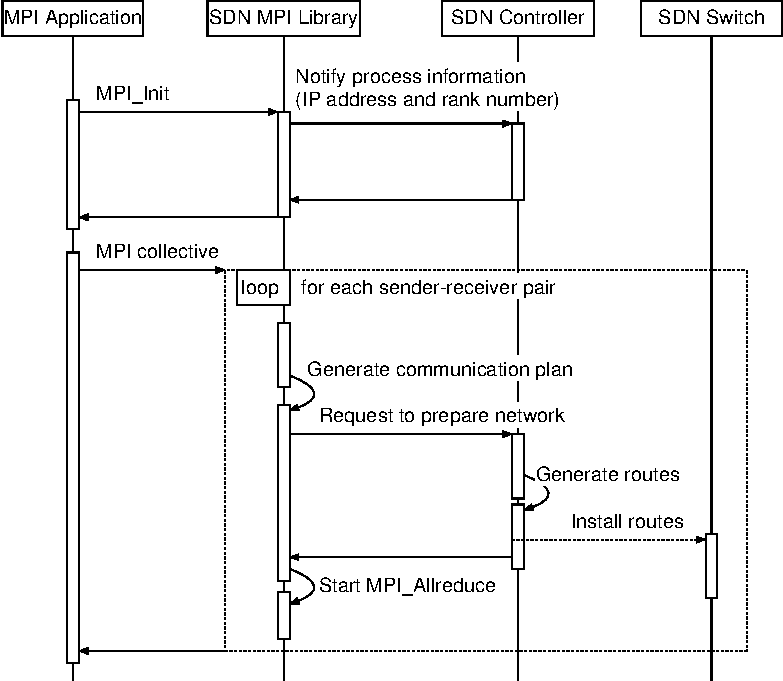
\includegraphics{sdn-mpi-sequence}
    \caption{The Sequence Diagram of the Proposed Framework}%
    \label{fig:proposal-sequence}
\end{figure}

When an MPI collective is called, the rank 0 process generates the
communication pattern of the MPI collective. This communication pattern is a
set of sender process and receiver process pairs during the MPI collective
communication. After the communication pattern is generated, this set is sent
to the SDN controller by the rank 0 process. As soon as the SDN controller
receives the communication pattern, it generates a route for each
sender-receiver pair. Subsequently, the SDN controller programs each
SDN-enabled switch so that the MPI packets are routed along the pre-generated
routes. After the entire communication pattern is processed, the MPI
collective is called to start the actual data transfer and computation for the
collective operation.

\subsection{Implementation of Collective Acceleration Framework Using SDN}

To realize the proposed framework, three modules that work as an integrated
system has been developed: LLDP daemon, SDN controller and SDN MPI library.
This section explains the implementation of these three modules in detail.

\subsubsection{LLDP Daemon}

Each compute node runs an LLDP daemon in the background. This daemon is
designed to emit LLDP packets containing hardware information periodically,
which are received by the SDN-enabled switches and used for topology
discovery. Some LLDP daemon implementations already exist. However, a new,
minimal daemon has been developed to easily add and tweak features so that it
can cooperate with the other programs composing the whole system.

The developed daemon detects all available network interfaces installed on a
computer and queries its interface index, MAC address and IP address.
This information is packed into a single LLDP packet and sent out from
each network interface periodically. The interval is set to one second in
this prototypical implementation to speed up the topology discovery.
However, it can be a longer period in practical systems so that its
topology does not change frequently.

As described above, the LLDP daemon emits a few hundred byte long packets to
the network every second. This traffic is considered to be small enough so
that it does not cause serious side effects on the actual MPI process, for
instance taking CPU time away from the application or consuming too much
bandwidth that could interfere with the MPI communication. Generating such
LLDP packets is also not a difficult task for a today's  computer, so the
impact to the application is considered to be ignorable.

\subsubsection{SDN Controller}

The SDN controller was developed on top  of Trema~\autocite{trema}, a
framework designed for easily developing OpenFlow controllers in the Ruby
language. It has the following four core functionalities:

\begin{enumerate}
    \item Generating routes for MPI collectives to mitigate link contention
          and installing the generated routes to SDN-enabled switches
    \item Detecting the topology and usage of the interconnect using LLDP
    \item Responding to Address Resolution Protocol~(ARP) requests from
          compute nodes to avoid broadcast storms
    \item Routing of non-MPI traffic such as ICMP and SSH
\end{enumerate}

The first functionality is topology detection. How detection is
performed is shown in Fig.~\ref{fig:lldp}. The controller periodically
requests every switch to send out an LLDP packet from each of their physical
ports (step~1 in Fig.~\ref{fig:lldp}). This LLDP packet contains two kinds of
information: datapath ID (a number that uniquely distinguishes the switches)
and port number (port index where the packet is sent out). Moreover, all
compute nodes also emit LLDP packets from the LLDP daemon described in the
previous section. The controller is notified of a LLDP packet arrival at a
switch. After that, it parses the packet to obtain the information on the
packet's origin, and then examines whether the packet came from a compute node
or an SDN-enabled switch. If the sender is a compute node, its MAC address and
interface index is acquired. Otherwise if the sender is a switch, its datapath
ID and port number is acquired (step~2). Using this information from its
neighbors, an adjacency list is generated (step~3). From this adjacency list,
a network topology graph is constructed, which is used in the route generation
and routing. If the packet is from a compute node, the source MAC address and
IP address are registered in a MAC/IP address translation table used in the
ARP responding functionality.

\begin{figure}
    \centering
    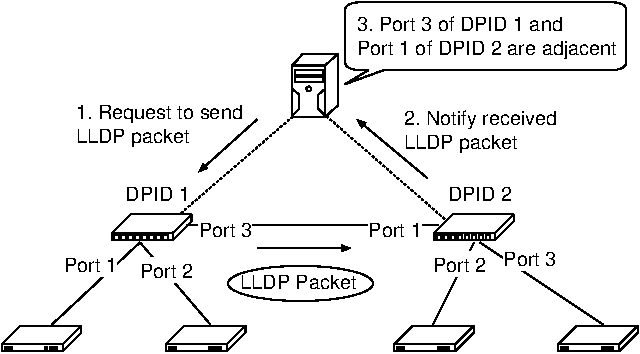
\includegraphics{lldp}
    \caption{Topology Detection using LLDP}%
    \label{fig:lldp}
\end{figure}

The second functionality is replying to ARP requests. ARP requests are L2
broadcast packet and therefore causes a \emph{broadcast storm} in a network
that contains a cycle. Since this chapter targets a network that has redundant
routes, the topology of the network is not a tree. Therefore, the network is
always cyclic. Thus, the controller instructs the switches to reply to the
received ARP request, instead of the compute node that has the corresponding
IP address. The IP address that corresponds to the MAC address is obtained
from the MAC/IP address translation table described above.

The third functionality is route generation and installation for MPI
collective communication. The route generation algorithm is implemented as a
pluggable module so that different algorithms can be specifically tailored for
each MPI collective.

% アルゴリズムの目的
Since this research focuses on accelerating MPI\_Allreduce, a route generation
algorithm targeting MPI\_Allreduce has been designed and implemented. The goal
of this route generation algorithm is to mitigate the interference between the
packet flows generated by the underlying point-to-point communication of
MPI\_Allreduce. In particular, the proposed algorithm tries to generate routes
so that the packet flows are evenly distributed among the redundant routes in
the interconnect. In other words, the proposed algorithm aims to minimize the
maximum number of packet flows sharing a link.

% 解の最適性についての議論
Note that this problem is a combinatorial optimization problem on a
multi-commodity flow network and thus requires heavy computation to find the
optimal solution. Meanwhile, the SDN controller needs to perform the route
generation every time an MPI collective is called as described in
Section~\ref{sec:iii-design}. Therefore, the proposed algorithm is designed to
be a heuristic algorithm based on a greedy strategy that quickly finds an
approximate solution rather than an optimal solution.

% アルゴリズムの基本的なアイディア
The basic idea behind this heuristic algorithm is to assign a route to each
point-to-point communication iteratively. At each iteration, the algorithm
selects a pair of a sender and a receiver and finds the least utilized route
between them. This is achieved by considering a weighted graph where the
weight of a link is equal to the total number of packet flows going through
the link, and then finding the shortest route between the sender process and
receiver process in this graph. Here, the \emph{Dijkstra} algorithm is used to
find the shortest route because of its speed and simplicity. After a route is
assigned, the weight of each link along the generated route is incremented.
This procedure is repeated for all sender-receiver pairs.

% 擬似コードを使った具体的な説明
Algorithm~\ref{lst:code-generate-route} is a pseudo-code for the algorithm.
First, an empty array \emph{routes} is initialized (line 1 in
Algorithm~\ref{lst:code-generate-route}). After that, the route search is
performed for each sender-receiver pair (line 4--7). The resulting route is
added to \emph{routes} (line 5) and the link weight (which is the number of
total routes that use that link) of each link is incremented (line 6--7).
After all routes are generated, these routes are installed to the SDN-enabled
switches.

\begin{algorithm}
    \SetKwData{Routes}{routes}
    \SetKwData{Nodes}{nodes}
    \SetKwData{Link}{link}
    \SetKwData{Links}{links}
    \SetKwData{Route}{route}
    \SetKwData{Sender}{sender}
    \SetKwData{Receiver}{receiver}
    \SetKwFunction{Dijkstra}{dijkstra}

    \Routes $\gets$ empty array\;
    \Nodes $\gets$ nodes in the topology graph\;
    \Links $\gets$ links in the topology graph\;

    \ForEach{(\Sender, \Receiver) $\in$ sender-receiver pairs}{%
        \Route $\gets$ \Dijkstra{\Nodes, \Links, \Sender, \Receiver}\;
        \ForEach{\Link $\in$ \Route}{%
            Increment weight of \Link\;
        }
    }

    \caption{Pseudocode of Route Generation}%
    \label{lst:code-generate-route}
\end{algorithm}

The fourth functionality is route generation and installation for
non-MPI traffic. For non-MPI traffic such as ICMP and SSH packets, the
SDN controller generates the minimum hop routes between compute nodes
and installs them on demand.

\subsubsection{SDN MPI Library}

An MPI application that wants to use the proposed framework must be linked
with the SDN MPI library. This library contains two classes of functions:
SDN\_MPI\_Init, which is an initialization function for the library, and
MPI collective functions prefixed with SDN\_MPI\_, which replace the
conventional MPI collectives with their SDN-enhanced versions.

The application is required to call SDN\_MPI\_Init when it launches. This
function opens a TCP connection with the SDN controller and notifies the IP
address and MPI rank number of the process that has called itself.

SDN\_MPI collectives are called by the application when it needs to perform
collective communication. Each SDN\_MPI collective generates the communication
pattern (set of sender process and receiver process pairs during the
collective communication) for the MPI application and sends the pattern to the
SDN controller.

\begin{figure}
    \centering
    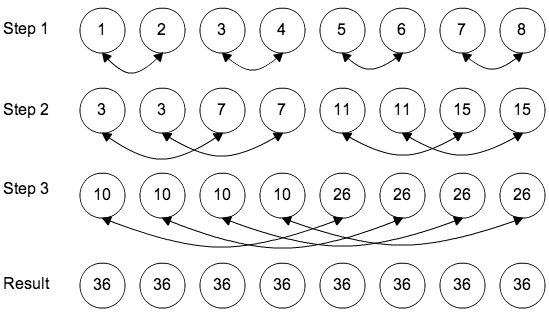
\includegraphics{recursive-doubling}
    \caption{Recursive Doubling Algorithm}%
    \label{fig:recursive-doubling}
\end{figure}

Several algorithms to realize the Allreduce operation have been
proposed~\autocite{Rabenseifner2004,Thakur2005,Kandalla2012,Ruefenacht2017}.
This research focuses on \emph{recursive doubling}~\autocite{Thakur2005},
since it requires more inter-node communication compared with other
algorithms, which means more room for optimization in terms of communication.
Figure~\ref{fig:recursive-doubling} illustrates how the recursive doubling
algorithm works. The recursive doubling algorithm requires $\log p$
communication steps where $p$ denotes the number of processes. For explanatory
purposes, the \emph{distance} between two MPI processes is defined as the
absolute difference of their rank numbers here. In the first step, processes
that are one distance apart exchange their data and perform the reduction
operation between the data that the process has originally held and with the
just exchanged data. In the second step, processes that are 2 distance apart
exchange their data, and in the $i$-th step, processes that are $2^{i - 1}$
distance apart exchange their data. The SDN MPI library memorizes all process
pairs that have to communicate and exchange data by following each step of the
recursive doubling algorithm. For each of those pairs, the library notifies
the SDN controller to prepare each route.

\section{Evaluation}\label{sec:iii-evaluation}

\subsection{Experimental Environment}

An experiment was conducted to compare the execution time of MPI\_Allreduce
accelerated with the proposed framework against conventional
MPI\_Allreduce. The experimental environment is illustrated in
Fig.~\ref{fig:experiment-environment}. This experiment was performed on
a real cluster system consisting of 28 compute nodes and 6 SDN-enabled
switches, which formed a two-tier fat-tree topology. The compute nodes and
SDN-enabled switches were all connected through Gigabit Ethernet links;
hence the interconnect was oversubscribed.

In addition to the network connecting the compute node and switches,
another network was prepared for control and management. This network
connects compute nodes, SDN-enabled switches and the SDN controller.
The interaction between the SDN controller and SDN switches is performed
via OpenFlow protocol with this management network. The compute node
that runs MPI's rank 0 process and the SDN controller also communicates
with this network. Other compute nodes were connected to the
management network as well, but those connections were not used in this
experiment.

CentOS 6.4 was installed on all computers including the compute nodes and
SDN controller. The SDN controller was developed using a SDN controller
framework Trema~\autocite{trema} 0.4.6 and Ruby 1.9.3. The SDN
MPI Library and the benchmark application were written in C and
compiled with gcc 4.4.7. As a representative of a conventional MPI,
Open~MPI~\autocite{Gabriel2004} 1.5.4 was used.

\begin{figure}
    \centering
    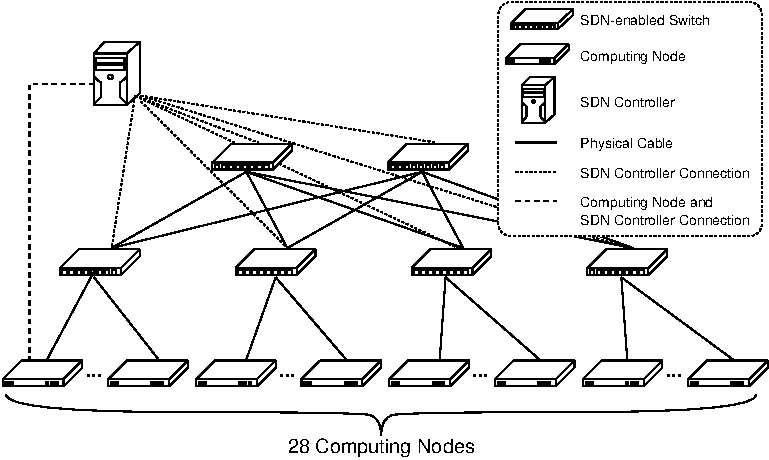
\includegraphics{sdn-mpi-exp-env}
    \caption{Experimental Environment}%
    \label{fig:experiment-environment}
\end{figure}

\subsection{Measurement Result}

A micro-benchmark that repeats MPI\_Allreduce 20
times and measures the average execution time of the function was used
for comparing the execution time of the proposed MPI\_Allreduce
with its Open~MPI counterpart.

Figure~\ref{fig:evaluation-8nodes} shows the measurement results using 8
nodes, where the horizontal axis indicates the message size and the
vertical axis shows the average time taken to execute
MPI\_Allreduce. The solid line and dashed line represent the
execution time of the proposed framework and Open~MPI implementation,
respectively. Figure~\ref{fig:evaluation-8nodes-normalized} shows the speedup
of MPI\_Allreduce accelerated using the proposed framework in comparison with
the Open~MPI implementation. The maximal speedup was 41\%.
Figure~\ref{fig:evaluation-16nodes} shows the result in the case of using 16
nodes. Figure~\ref{fig:evaluation-16nodes-normalized} indicates the speedup of
the proposed MPI\_Allreduce. It shows that the proposed framework succeeded to
realize a 56\% speedup at maximum.

\begin{figure}
    \centering
    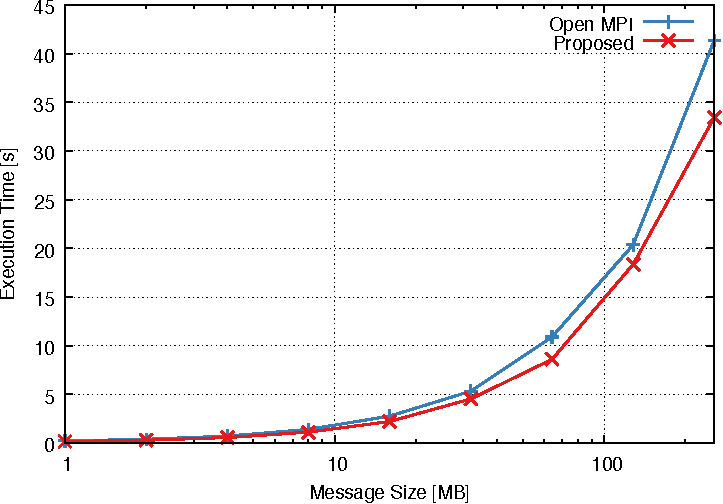
\includegraphics{allreduce_8nodes}
    \caption{Comparison of Execution Time of MPI\_Allreduce (8 Compute Nodes)}%
    \label{fig:evaluation-8nodes}
\end{figure}

\begin{figure}
    \centering
    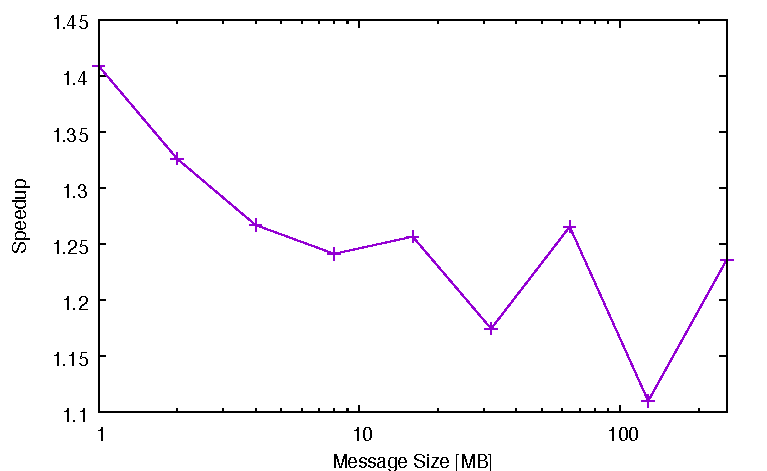
\includegraphics{allreduce_8nodes_speedup}
    \caption{Speedup of Proposed MPI\_Allreduce (8 Compute Nodes)}%
    \label{fig:evaluation-8nodes-normalized}
\end{figure}

\begin{figure}
    \centering
    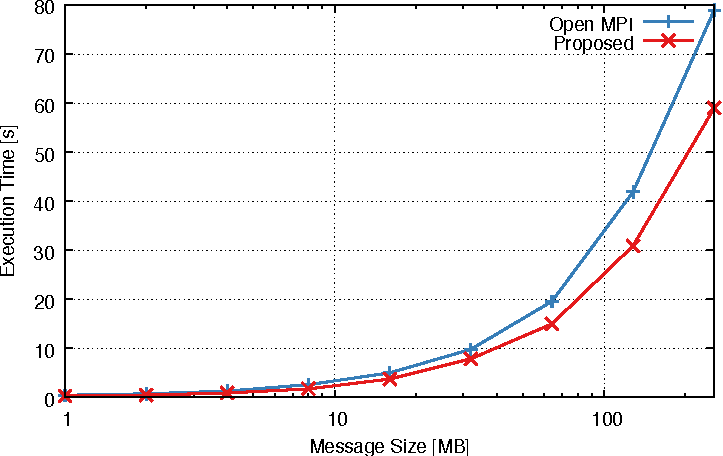
\includegraphics{allreduce_16nodes}
    \caption{Comparison of Execution Time of MPI\_Allreduce (16 Compute Nodes)}%
    \label{fig:evaluation-16nodes}
\end{figure}

\begin{figure}
    \centering
    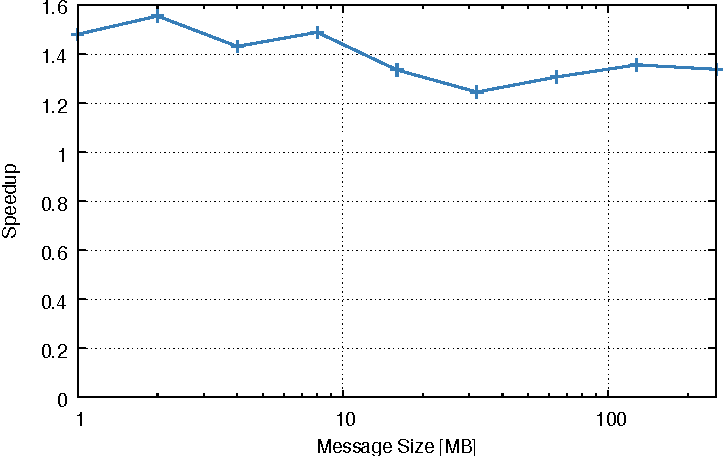
\includegraphics{allreduce_16nodes_speedup}
    \caption{Speedup of Proposed MPI\_Allreduce (16 Compute Nodes)}%
    \label{fig:evaluation-16nodes-normalized}
\end{figure}

Both Figs.~\ref{fig:evaluation-8nodes-normalized}
and~\ref{fig:evaluation-16nodes-normalized} clearly show that MPI\_Allreduce
accelerated with the proposed framework is consistently faster than the Open
MPI implementation. However, some fluctuation of the speedup is also observed.
This fluctuation of performance is considered to be caused by the
non-deterministic aspect of the network. For example, queueing and scheduling
of packets at compute nodes and switches, TCP congestion control, and OS noise
heavily affect the time it takes for each packet to travel through the
network. Such variation in the latency of each point-to-point communication
significantly impacts the execution time of a collective communication. A
larger number of benchmark runs is expected to exhibit a constant speedup
ratio.

\section{Related Work}\label{sec:iii-related-work}

There have been many research works related to MPI\@. Since MPI is merely a
specification for standard APIs for parallel programming, several algorithms
for collective operations have been proposed and implemented targeting several
network technology. As a representative example of such works,
MVAPICH~\autocite{mvapich} can be raised. MVAPICH is an MPI implementation
targeting InfiniBand, which most of high-performance computing systems ranked
in Top500 have adopted. Sur \emph{et al.}~\autocite{Sur2011} designed an MPI
library by leveraging novel InfiniBand-offered features. They explored new
architectures from a system point of view and new programming paradigms from
an application point of view to keep scaling out applications on more powerful
computing systems. Jiuxing \emph{et al.}~\autocite{Jiuxing2004} also
investigated an MPI communication protocol focusing on RDMA operations in
InfiniBand. The approach of this research has some points in common in terms
that this research also aims to benefit from the features of the underlying
network. However, this research leverages Software-Defined Networking instead
of InfiniBand from the purpose of investigating the feasibility of dynamic
control of network from an application point of view.

Researchers have attempted to elaborate algorithms for MPI collective
operations. Optimized algorithms have been proposed for
MPI\_Alltoall~\autocite{Bruck1997},
MPI\_Reduce\_scatter~\autocite{Iannello1997}, MPI\_Reduce and MPI\_Allreduce.
Most of the optimized algorithms are specialized either for latency or
throughput, so switching multiple algorithms depending on the message size or
process number makes the MPI implementation behave faster for various message
sizes and process numbers~\autocite{Thakur2005}.

Another approach is to offload the communication or computation of collective
communication operations to hardware. For example, the
\emph{K-computer}~\autocite{Yokokawa2011} has a hardware module called
\emph{Tofu Barrier Interface}~\autocite{Ajima2012} on all nodes. This module
executes Barrier, Broadcast, Reduce and Allreduce collective operations in
hardware instead of software. However, this approach does not mitigate
the congestion on links.

Past works including existing MPI implementations have been successful in
switching between multiple algorithms depending on message size, node number,
\emph{etc.} to accelerate collective communication in MPI\@. Using such a
mechanism, some estimation of the threshold value for parameters like message
size, node number, \emph{etc.} is essential. Pje\v{s}ivac-Grbovi\'{c} \emph{et
al.}~\autocite{PjesivacGrbovic2007} compared several parallel communication
models that are frequently used for dynamically estimating the threshold
values. In contrast, the current implementation of the proposed framework
always uses recursive doubling for executing MPI\_Allreduce. Therefore, the
proposed framework has a disadvantage in the cases where small data size is
treated on MPI\_Allreduce and thus the latency is more respected than the
bandwidth. For this disadvantage, automatic switching of algorithms that
leverages estimation models is planned to be introduced.

The Fabric Collective Accelerator (FCA)~\autocite{fca} is a product by
Mellanox Technologies with the target of accelerating collective
communication on clusters with InfiniBand interconnect. FCA accelerates
collective communication by offloading computations to an InfiniBand
Host Channel Adapter (HCA). It also optimizes communication flow
according to job and topology. FCA optimizes collective tree and rank
placement to control communication flow. In contrast, the proposed
framework is capable of adaptively reconfiguring the network itself,
which is more flexible. FCA also requires InfiniBand hardware, but this
research focuses on a commodity Ethernet network.

Furthermore, there have been many research reports focusing on adaptive
use of networks for high-performance computing. Geoffray \emph{et
al.}~\autocite{Geoffray2008} proposed an adaptive routing method on Myrinet
and the above-mentioned literature~\autocite{Jiuxing2004} explored the
adaptive use of multiple independent networks on InfiniBand. This research also
aims for a dynamic use of the underlying interconnection network, but differs
in the fact that this research attempted to use a different interconnection
network.

\section{Conclusion}\label{sec:iii-conclusion}

This chapter has attempted to reduce the execution time of MPI
collectives by dynamically controlling the packet flow in the interconnect
using Software-Defined Networking~(SDN).
By using SDN, this research  has proposed a novel framework for accelerating
collectives that can effectively make use of redundant routes by having SDN
interact with the communication pattern of collectives. A system of three
modules cooperating together has been designed and implemented to realize the
proposed framework. The evaluation conducted in this chapter showed that the
proposed framework speeds up the execution time of MPI\_Allreduce for 56\% at
most compared with a conventional implementation of MPI\_Allreduce. This
result confirms the superiority of the proposed framework over conventional
methods.

Several issues to tackle have remained for the realization of practical
and useful collective acceleration framework leveraging SDN\@.
The first issue is the support for multiple processes on a single compute
node. On modern computing platforms where multiple cores are implemented in a
single compute node, the assumption set in this preliminary stage of this
research is neither practical nor realistic. Therefore, intra-node
communication for pure MPI jobs needs to be considered by integrating
kernel-assisted communication such as KNEM~\autocite{Goglin2013} or Cross
Memory Attach~(CMA) with the proposed method. Also, computing paradigms such
as the hybrid use of OpenMP with MPI must be considered for enhancing
practicality. Also, other implementations of MPI such as
MVAPICH~\autocite{mvapich} are essential for investigating the practicality
and usefulness of SDN\@.

The second issue regards the necessity of additional experiments on a
larger scale environment. This chapter has verified the feasibility and
possibility of the proposed framework through the experiments using a simple
prototypical implementation. However, because OpenFlow switches were expensive
and thus only a small-scale cluster was available, only a limited number of
experiments in a small cluster environment could be conducted. Therefore,
further experiments on a larger scale environment are essential for the
evaluation of future scalability.

The third issue is the scalability issue caused by the SDN controller.
Since the current implementation requires communication between MPI processes
and SDN controller and route generation for each MPI communication request,
the SDN controller might become a scalability bottleneck on larger
environments. Therefore, the IP address and MPI rank number for each process
need be cached in the SDN controller. Furthermore, the current implementation
needs to be enhanced so that only the root process interacts with the SDN
controller and conveys information of all participating processes in the
collective communication.
